\documentclass[12pt,a4paper]{article}

\usepackage[utf8]{inputenc}
\usepackage[greek,english]{babel}
\usepackage{alphabeta} 

\usepackage{amsmath}
\usepackage{mathtools}

\usepackage{algorithm}
\usepackage{algpseudocode}

\usepackage[pdftex]{graphicx}
\usepackage[top=1in, bottom=1in, left=1in, right=1in]{geometry}

\linespread{1.06}
\setlength{\parskip}{8pt plus2pt minus2pt}

\widowpenalty 10000
\clubpenalty 10000

\newcommand{\eat}[1]{}
\newcommand{\HRule}{\rule{\linewidth}{0.5mm}}

\usepackage[official]{eurosym}
\usepackage{enumitem}
\setlist{nolistsep,noitemsep}
\usepackage[hidelinks]{hyperref}
\usepackage{cite}
\usepackage{lipsum}
\usepackage{amsmath}
\usepackage{algorithm}
\usepackage[noend]{algpseudocode}

\begin{document}

%===========================================================
\begin{titlepage}
\begin{center}

% Top 

\includegraphics[width=0.40\textwidth]{Indian_Institute_of_Technology,_Indore_Logo.png}~\\[2cm]


% Title
\HRule \\[0.4cm]
{ \LARGE 
  \textbf{CS 309 \\ Parallel Computing}\\[0.4cm]
  \emph{Parallel Algorithms for Evaluation of Matrix Polynomials}\\[0.4cm]
}
\HRule \\[1.5cm]



% Author
{ \large
  Course Instructor: Dr. Chandresh Kumar Mourya\\[0.8cm]
  Purnadip Chakrabarti (190002048) \\[0.1cm]
  Garvit Galgat (190001016) \\[0.1cm] 
  Vaibhav Chandra (190001065) \\[0.1cm]
  Peddamallu Bhuvana Sree (190001046) \\[0.1cm]
}

\vfill


% Bottom
{\large \today}
 
\end{center}
\end{titlepage}

\newpage

%===========================================================
\tableofcontents
\addtocontents{toc}{\protect\thispagestyle{empty}}
\newpage
\setcounter{page}{1}

%===========================================================
%===========================================================
\section{Introduction}\label{sec:intro}

The problem statement that we solve in this paper is that given a real or complex matrix $A$ and a polynomial $$q(x) = \sum_{i=1}^{d} c_{i}x^{d} = c_{0} + c_{1}x + c_{2}x^{2} + ... c_{d}x^{d}$$ with real or complex coefficients $c_{0},c_{1},..c_{d}$ , we wish to compute the matrix polynomial $q(A)$. The brute-force technique to solve this involves computing all powers of matrix A and then performing $O(d)$ matrix multiplications and $O(d)$ matrix additions. If the time complexity of matrix multiplication is $O(n^{\omega})$ (where $A$ is a $n \times n$ matrix) then the time complexity of the naive algorithm is $O(n^{\omega}d)$. This is quite bad especially for large matrices and high degree polynomials. Here, $\omega$ = 3 for naive matrix multiplication and $\omega$ $\approx$ 2.7 for Strassen matrix multiplication. Although Strassen matrix multiplication is asymptotically more efficient, we have used naive matrix multiplication because the constant term of Strassen matrix multiplication is quite large and naive matrix multiplication is easily parallelizable.  

However, there exists some optimal algorithms to evaluate matrix polynomials in lesser time complexity. We are going to use two algorithms for the same
\begin{enumerate}
    \item Paterson Stockmeyer Algorithm
    \item Parlett Recurrence Algorithm
\end{enumerate}

Paterson Stockmeyer algorithm is a robust algorithm which re-orders the polynomial and reduces the dependence of time complexity on the degree of the polynomial. It's overall time complexity is $O(n^{3}\sqrt{d})$. The details of the theory of Paterson Stockmeyer algorithm are given in section 2. The implementation and parallelization techniques are described in section 3.

Parlett Recurrence algorithm is even more efficient algorithm with time complexity $O(n^{3})$. But, it is numerically unstable for some cases which will be illustrated in section 2. This numerical instability can be removed using diagonal block re-orddering of Schur decomposed form of the input matrix. But, the implementation of the same is quite involved both algorithmically and theoretically and hence, we have left the same for future developments of the project. Also, there are some more edge cases which are specific to the implementation of the internal components of Parlett Recurrence algorithm. Moreover, the constant term of the time complexity is very high. Hence, this algorithm works better than Paterson Stockmeyer algorithm only for large matrices and high degree polynomials. We will use this fact to design our overall algorithm which will be described in section 3.

\newpage
In our implementation, we are going to use a blocked version of Parlett Recurrence algorithm to take advantages of our parallelized matrix multiplication algorithm which will be described in section 3. There are 2 components which are integral part of blocked Parlett Recurrence algorithm which are as follows:
\begin{enumerate}
    \item Schur Decomposition
    \item Sylvester Equation Solver
\end{enumerate}

Schur Decomposition involves a numerical method known as $QR$ method. For this, we need to perform a QR decomposition. There are various ways to perform the same. To name a few, Gram-Schmidt method, Householder method, Given's rotation method are used for the same. We have chosen to incorporate Given's rotation technique to compute QR decomposition. There are some edge cases for which Given's rotation matrix can't be computed but this method has a lot of scope for parallelization. Since our main focus is on parallelization of the matrix polynomial evaluation, we have preferred Given's rotation technique over other techniques which have far less scope of parallelization. Details of all these sub-components will be explained in section 2 and 3.

Sylvester Equation Solver involves various components some of which are computation of Kronecker product and Gauss Elimination. Details of the same are described in section 2 and 3. Finally, for blocked Parlett Recurrence algorithm, we first compute the Schur Decomposed form of the input matrix and then we apply Sylvester Equation Solver over all the blocks of Schur decomposed form. These details are explained in section 2 and 3.

\newpage
\section{Theory}\label{sec:lit-rev}

\subsection{Paterson Stockmeyer Algorithm}

The original polynomial $q(A)$ is written as 
$$q(A) = \sum_{i=1}^{d} c_{i}A^{d} = c_{0}I + c_{1}A + c_{2}A^{2} + ... c_{d}A^{d}$$
Now, according to the algorithm, we choose two integers $p$ and $s$ and we re-write $q(A)$ as
$$q(A) = (c_{0}I + c_{1}A + .... c_{p-1}A^{p-1})(A^{p})^{0}$$ $$ + (c_{p}I + c_{p+1}A + .... c_{2p-1}A^{p-1})(A^{p})^{1}$$ $$\vdots$$ $$(c_{(s-1)p}I + c_{(s-1)p+1}A + .... c_{sp-1}A^{p-1})(A^{p})^{s-1}$$
\\
Basically, $q(A)$ is rewritten as a polynomial in $A^{p}$ and all the coefficients of this polynomial are themselves a polynomial in $A$ with degree at most $p-1$. It is quite obvious that if these two expressions are same then 
$$c_{i} = 0 \hspace{0.25cm} \forall \hspace{0.25cm} i > d$$ 
Although we can choose any two integers $p$ and $s$, it is observed that the algorithm gives the best time complexity when $s \simeq p \simeq \sqrt{d}$. It is particularly this case when we get overall time complexity as $O(n^{3}\sqrt{d})$. This can be proved theoretically as well. Clearly, the highest degree of the rearranged polynomial must be greater than or equal to $d$. So, 
$$p(s-1) + p-1 \geq d$$
$$ps \geq d+1$$
From this equation, we can clearly observe that if $p \simeq s \simeq \sqrt{d}$ then we will have to do least number of extra computations. Now, for computing this re-arranged polynomial, we will have to compute all powers of $A$ till $p$. We have developed an efficient algorithm to do this and this has been described in section 3. Then, we apply Horner's algorithm to compute the complete polynomial. Details of Horner's algorithm are discussed in section 3.
\newpage
\subsection{Schur Decomposition}

There is a theorem in linear algebra which states that for any complex $n \times n$ square matrix $A$, we can write $A$ as
$$A = Q^{H}TQ$$
where $Q$ is a unitary matrix and $T$ is an upper triangular matrix with all eigen values of $A$ in it's diagonal. $Q^{H}$ denotes the conjugate transpose of unitary matrix $Q$. This decomposition is known as Schur Decomposition and the upper triangular matrix $T$ is called Schur form of $A$. The matrix $A$ can have complex eigen values too. But, in our implementation we have used a modified version of the Schur form. The modified Schur form is called Real Schur form of $A$ which is quasi-upper triangular in nature. All the diagonal blocks of real Schur form of $A$ are either $1 \times 1$ for real eigen values or $2 \times 2$ for complex eigen values. If we write the $2 \times 2$ diagonal block as 
$$\begin{bmatrix}a & b \\ c & d \end{bmatrix} \hspace{0.5cm}  a, b, c, d \in \mathbb{R},\hspace{0.25cm} b < 0, \hspace{0.25cm} a = d$$
then the two complex eigen values associated with this matrix are $a \pm i\sqrt{\mid bc \mid}$. \\ In our implementation, we have used a numerical method known as $QR$ method to compute the Schur decompositon. In this numerical method, we define $A_{k}$ as the upper triangular matrix generated after $k^{th}$ iteration of $QR$ method. In $k^{th}$ iteration, we first perform QR decomposition of $A_{k-1}$ to obtain $A_{k-1} = Q_{k-1}R_{k-1}$. It is to be noted that $QR$ decomposition yields a unitary matrix $Q$ and an upper triangular matrix $R$. Now, we obtain by $A_{k} = R_{k-1}Q_{k-1}$. We start the iterations with $A_{0} = A$. According to a theorem in linear algebra, after infinite iterations, $A_{k}$ will converge to a quasi-upper triangular matrix (as defined in section 1) which will have all eigen values of matrix $A$ on it's diagonal in the form of $1 \times 1$ and $2 \times 2$ blocks. The proof of this is quite involved and since it is not the focus of our project, we are omitting the proof from this documentation. \\ Now that we have obtained the quasi upper triangular matrix $T$ from $A_{k}$, we also have to compute the unitary matrix $Q$. Now, we can write the following equations
$$A_{0} = Q_{0}R_{0}$$
$$A_{1} = R_{0}Q_{0}$$
Since $Q_{0}$ is a unitary matrix from the definition of $QR$ decomposition, we can write $Q_{0}^{H}Q_{0} = I$. Using this fact,
$$A_{1} = IR_{0}Q_{0} = Q_{0}^{H}Q_{0}R_{0}Q_{0}$$
$$\implies A_{1} = Q_{0}^{H}(Q_{0}R_{0})Q_{0}$$
$$\implies A_{1} = Q_{0}^{H}A_{0}Q_{0}$$
Using similar arguments for $A_{2}$, we can write
$$A_{2} = Q_{1}^{H}A_{1}Q_{1}$$
\newpage
Now, replacing $A_{1}$ with the the expression we just calculated, we get
$$A_{2} = Q_{1}^{H}Q_{0}^{H}A_{0}Q_{0}Q_{1}$$
$$\implies A_{2} = (Q_{0}Q_{1})^{H}A_{0}(Q_{0}Q_{1})$$
Now, if we write the expression in a similar manner for $A_{k}$, we will get
$$A_{k} = (Q_{0}Q_{1}...Q_{k-1})^{H}A_{0}(Q_{0}Q_{1}...Q_{k-1})$$
$$\implies A_{0} = (Q_{0}Q_{1}...Q_{k-1})A_{k}(Q_{0}Q_{1}...Q_{k-1})^{H}$$
Now, we know that $A_{0} = A$ and $A = Q^{H}TQ$. Here $Q$ was a unitary matrix and $T$ was a quasi upper triangular matrix. Now, if we compare this expression with the expression we just computed then we see that LHS is the same for both of them and in RHS, $A_{k} = T$. Moreover, product of 2 unitary matrices is also a unitary matrix. So, we can say that 
$$Q = (Q_{0}Q_{1}...Q_{k-1})^{H}$$
Hence, we have obtained the expression for $Q$ matrix. This $Q$ matrix will be required in Parlett Recurrence method. Now, the only part left is the method for $QR$ decomposition. As mentioned in the introduction, there are various ways to perform $QR$ decomposition. Since our main focus is on parallelization of matrix polynomial evaluation, we picked up Given's rotation technique which has a lot of scope for parallelisation. 

The theory of Given's rotation involves quite a deal of geometry. Hence we are omitting the details of the proofs and we will directly explain the algorithm. Now, a Given's matrix can be defined as
$$G(i, j, \theta) = 
\begin{bmatrix} 
1 & ... & 0 & ... & 0 & ... & 0 \\
\vdots & \ddots & \vdots & & \vdots & & \vdots \\
0 & ... & c & ... & -s & ... & 0 \\
\vdots & & \vdots & \ddots & \vdots & & \vdots \\
0 & ... & s & ... & c & ... & 0 \\
\vdots & & \vdots & & \vdots & \ddots & \vdots \\
0 & ... & 0 & ... & 0 & ... & 1 
\end{bmatrix}$$
where $c = cos\theta$ and $s = sin\theta$. Now, according to the algorithm, given a matrix $A$, we want to make it upper triangular. This is possible if we make the numbers below the diagonal as $0$. Here is where Given's matrix will help us. Let's say that we want to convert $A_{2, 1}$ to $0$. In this case, we will find such a Given's matrix such that $G(i, j, \theta)A$ has the entry as $0$ at $(2, 1)$ index. Here, we will fix $i = 2, j = 1$ and we have to calculate $\theta$ such that we get the desired result. We came up with an formula which can be proved easily by matrix multiplication.
$$\theta = tan^{-1}(-A_{ij} / A_{jj})$$
\newpage
Now, we will compute the Given's matrices for all the indices below the diagonal. Let's denote these Given's matrices as $G_{21}, G_{31}...G_{n,(n-1)}$. So, for the $QR$ decomposition, we can write
$$R = G_{n,(n-1)}...G_{31}G_{21}A$$
$$Q = (G_{n, (n-1)}...G_{31}G_{21})^{H}$$
The proof of this is quite elaborate and is omitted because our main focus lies on the algorithm and its parallelization. Hence, this completes the theory of all the sub-components of Schur Decomposition. The implementation and parallelization details will be provided in section 3.

\subsection{Sylvester Equation Solver}

An equation of the form $$AX - XB = C$$ is known as a Sylvester equation. Here $A$ is a square matrix of dimension $p \times p$(say) and $B$ is a square matrix of dimension $q \times q$(say). $C$ is a matrix of dimension $p \times q$ and $X$ is a $p \times q$ matrix which needs to be computed. There exists a standard solution for X for such an equation. This equation can be re-written as $$Kx=b$$ where $K=I_q\bigotimes A- I_p\bigotimes B$ (Here $\bigotimes$ denotes Kronecker product and $I_c$ is a c x c identity matrix) and $$b=\begin{bmatrix}c_1 \\ c_2 \\ . \\ . \end{bmatrix}$$ 
where $c_1,c_2,...,c_n$ are columns of C from right to left. Similarly, we can write $x$ as
$$x=\begin{bmatrix}x_1 \\ x_2 \\ . \\ . \end{bmatrix}$$
where $x_1, x_2, ..., x_n$ are columns of X from right to left. Here, $x$ can be calculated by using Gauss Elimination method. We haven't given the details of Gauss Elimination as it is a pretty well known and standard algorithm to solve system of linear equations. X can then be calculated by reverse stacking the columns of x. 
This is to be noted that the solution $X$ of the Sylvester equation is unique if and only if the matrices $A$ and $B$ have no common eigen values. This is the primary reason behind the numerical instability of Parlett Recurrence algorithm. The application of Sylvester Equation will be seen in next section.The implementation and parallelization details will be given in section 3.

\subsection{Blocked Parlett Recurrence}
The idea behind Parlett Recurrence is to first perform Schur Decomposition to get $T$ from $A = Q^{H}TQ$. Our original problem is to compute $q(A)$ where $A$  is the input matrix. Now, we will compute $q(T)$ first and then we will find $q(A)$ by
$$q(A) = Q^{H}q(T)Q$$
Here, $T$ will have diagonal blocks of dimension either $1 \times 1$ or $2 \times 2$. Accordingly, we will divide this quasi-upper triangular matrix into blocks. Diagrammatically, an example of division into blocks can be shown like the following figure

\begin{figure}
    \centering
    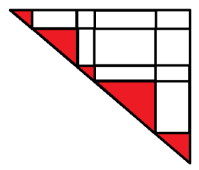
\includegraphics[width=0.30\textwidth]{Blocks.png}
    \caption{Block Partitioning}
\end{figure}

Here, red blocks denote the diagonal blocks and the white blocks are the off-diagonal blocks. Now, to compute $q(T)$, we have two steps. Here, we denote $F_{ij}$ as the computed function for the block $T_{ij}$ placed at $(i, j)$ location in the matrix $T$. So, first step is to compute the polynomial $F_{ii}$ for all the diagonal blocks $T_{ii}$. The second step is to compute the polynomial for the off-diagonal elements of $T$.

$F_{ii}$ can be calculated for all diagonal blocks efficiently using Paterson-Stockmeyer algorithm as subroutine. Now, the original relation proposed by Parlett is
$$f_{ij} = \frac{f_{ii}t_{ij} - t_{ij}f_{jj}}{t_{ii} - t{jj}} + \sum_{k=i+1}^{j-1}\frac{f_{ik}t_{kj} - t_{ik}f_{kj}}{t_{ii} - t_{jj}}$$
Here, $t_{ij}$ and $f_{ij}$ represents the individual elements of the $T$ and $q(T)$ matrix respectively. From this relation, this is pretty clear that we can't calculate $f_{ij}$ if $t_{ii} = t_{jj}$. This scenario will happen if the input matrix $A$ has repeated eigen values because in that case two entries of the diagonal of real Schur form of $A$ will be equal. This is the reason we said that Parlett Recurrence method is numerically unstable for cases when input matrix $A$ has repeated eigen values.

However, rather than computing each entry seperately, we have implemented a blocked version of the Parlett Recurrence so that we can take advantages of our parallelized matrix multiplication algorithm. But, this version also suffers from repeated eigen value problem because Sylvester Equation can't give unique solution in this case. 
\newpage
The blocked Parlett recurrence relation to calculate $F_{ij}$ can be written as follows 
$$T_{ii}F_{ij} - F_{ij}T_{jj} = F_{ii}T_{ij} - T_{ij}F_{jj} + \sum_{k=i+1}^{j-1}(F_{ik}T_{kj} - T_{ik}F_{kj})$$ 

 Now, this is a Sylvester Equation where we have to compute $F_{ij}$. It can be easily noticed that each off-diagonal block $F_{ij}$ is only dependent on values of blocks to the left of it and below it. Since RHS must be known for solving this Sylvester equation, we have to compute these blocks before computing $F_{ij}$. There emerge two ways to calculate $F$ matrix:
\begin{enumerate}
    \item Block diagonal partitioning: If we define diagonal $d'$ to consist of all $F_{ij}$ blocks for which $j = i + d'$ then each diagonal $d'$ is only dependent on diagonals $d''<d'$ (diagonals to the left of d). Blocks within each diagonal can be calculated independently of each other which means they can all be calculated parallely quite efficiently.  
    \vspace{0.5cm}
    \item Block column partitioning: We can divide $T$ into blocks column-wise and calculate them in appropriate order sequentially from left to right. 
\end{enumerate}

We have chosen block diagonal partitioning due to its rather straightforward implementation and more explicit parallelization than column partitioning.

\newpage
\begin{figure}
    \centering
    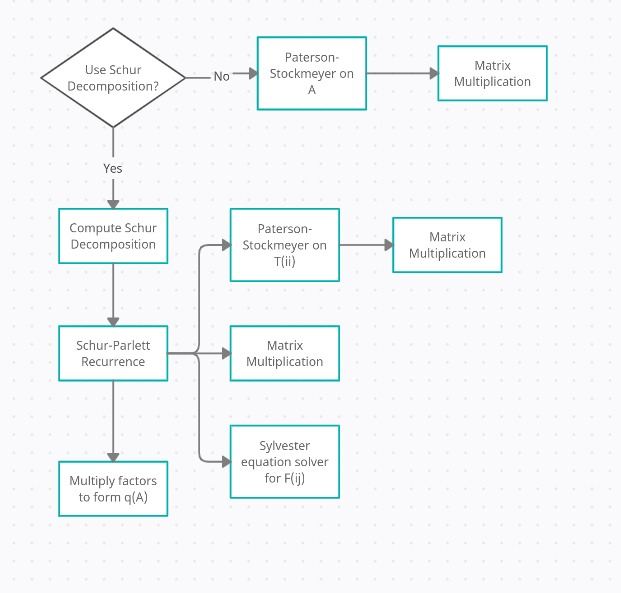
\includegraphics[width=0.7\textwidth]{flowchart.jpeg}
    \caption{Algorithm Overview}
\end{figure}
\section{Implementation and Parallelization}

We have implemented the algorithm from scratch using C++ 17 compiled on GNU G++ compiler. OpenMP was used for the development of parallel algorithms. 



\subsection{Paterson Stockmeyer Algorithm}
First step is to compute all powers of $A$ till power $p$. The naive way to compute and store these matrices involves p matrix multiplications which is quite expensive. However, we have come up with an efficient algorithm which is as follows:

\begin{algorithm}
\caption{Computing powers of $A$}\label{alg:cap}
\begin{algorithmic}[1]
\State Compute powers $A^{2}$, $A^{4}$, ..., $A^{2^{floor({log_{2}^{p}})}}$
\State For remaining even powers, compute its decomposition in terms of already computed powers and multiply the respective matrices
\State For all odd powers take the even power which is 1 less than it and then multiply that matrix with $A$
\end{algorithmic}
\end{algorithm}



In this algorithm, we can compute all the powers of $A$ which are not a power of 2 in parallel. Now, we present the Horner's method for Paterson Stockmeyer algorithm which is as follows: 

% yaha PS ka code chipka
\begin{algorithm}
\caption{Paterson-Stockmeyer Polynomial Evaluation}\label{euclid}
\begin{algorithmic}[1]
\State Q = 0
\State \text{Calculate and store A, $A^{2}$,..., $A^{p-1}$}
 \For{\textt{q = 0 : s-1}}
     \State {Q_p = {$c_{p.q}.I + c_{p.q+1}.A + c_{q.p+p-1}.A^{p-1}$}}
     \State {Q = {$Q.A^p + Q_p$} \Comment{Horner's Method}
\EndFor
\end{algorithmic}
\end{algorithm}
\newpage
The coefficients are the polynomials in $A$. The computation of each coefficient is parallelised in each iteration. 

\subsection{Schur Decomposition}

The algorithm to compute QR decomposition is as follows

\begin{algorithm}
\caption{QR Decomposition}\label{euclid}
\begin{algorithmic}[1]
\State $R$ = $A$
\State \text{$Q^{T}$ = $I$}
 \For{\textt{i = 1 : size}}
    \For{\textt{j = 0 : i}}
        \State {$G$ = ComputeGiven($R_{ij},R_{jj}$)}
        \State {$Q^{T} = GQ^{T}$}
        \State {$R=GR$}
    \EndFor
\EndFor
\State {return $Q,R$}
\end{algorithmic}
\end{algorithm}


Now, we can parallelize the above algorithm. We can observe that computation of two Given's matrices $G_{i_{1}j_{1}}$ & $G_{i_{2}j_{2}}$ and their multiplication to obtain $Q$ and $R$ can be done in parallel if $i_{1} \neq i_{2}$ and $j_{1} \neq j_{2}$. This is because we are applying given's rotation on a matrix which is the output of another given's matrix. So, if we want to parallelise these multiplications, we need to make sure that the input of a given's rotation is the output of another given's rotation. This is a serious hindrance for parallelization but we have worked out a solution for this. We notice that in one given's rotation only two rows are affected. So if we apply given's rotations for two different pairs of rows then we can parallelise the multiplications. So, we have developed a strategy in which we compute and multiply given's matrices for alternate positions on the diagonals of the matrix. For more clarity, the following diagram is attached in which the order of execution of the cells are given. If some cell has the value 5 then we are saying that in 5th iteration, that cell will become 0 after multiplying with respective Given's matrix.

\begin{figure}
    \centering
    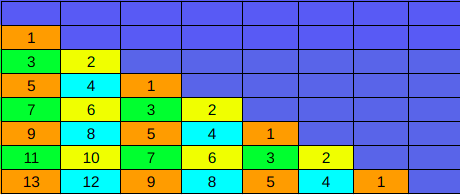
\includegraphics[width=0.70\textwidth]{givens.png}
    \caption{Order of Execution}
\end{figure}

\begin{algorithm}
\caption{Schur Decomposition}\label{euclid}
\begin{algorithmic}[1]
\State \text{$Q_f$ = I}
 \For{\textt{i = 0 : numberOfIterations}}
     \State {$Q,R$ = QRDecomposition($A$)}
     \State {$A = RQ$}
     \State {$Q_f$ = $Q_fQ$}
\EndFor
\State {return {$Q_f^T$,$A$}}
\end{algorithmic}
\end{algorithm}
There is no overall parallelization in QR method but we have used several parallel subroutines like matrix multiplication etc.
\subsection{Sylvester Equation Solver}

Sylvester Equation Solver involves computing Kronecker product and Gauss Elimination as sub-routines. The algorithm is as follows.

\begin{algorithm}
\caption{Sylvester Equation Solver}\label{euclid}
\begin{algorithmic}[1]
\State \text{$K=I_q\bigotimes A- I_p\bigotimes B$}
\State {$b$ = Col($C$)}
\State {$x$ = gaussElimination(K,b)}
\State {Obtain $X$ from $x$}
\end{algorithmic}
\end{algorithm}

We have parallelized both Kronecker product computation and Gauss Elimination. In Kronecker product computation, every entry of the output matrix can be computed independently and hence is done parallely. In Gauss Elimination, when we try to make the elements below the diagonal 0, we notice that we can simultaneously perform elementary row transformations for all the entries in a column below the diagonal. Hence, we have parallelized Gauss elimination in this manner. Apart form these two sub-routines, \textit{column stacking} and \textit{reverse column stacking} sub routines are also parallelized.

\newpage
\subsection{Blocked Parlett Recurrence}

As already mentioned in section 2, we have performed block diagonal partitioning to compute the off diagonal elements of $q(T)$. In a diagonal of blocks, all blocks can be computed parallely because $F_{ij}$ depends on the computed values to the left and bottom of it only.
Diagramatically, we can represent the partitioning as


\begin{figure}
    \centering
    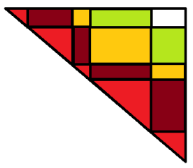
\includegraphics[width=0.30\textwidth]{Sylvester_blocks.png}
    \caption{Block Diagonal Partitioning}
\end{figure}

In the figure all the blocks of same color can be computed in parallel. Hence, we have deployed the same strategy to parallelize computations of off-diagonal elements. 

\begin{algorithm}
\caption{Blocked Parlett Recurrence}\label{euclid}
\begin{algorithmic}[1]
\State {$F_{ii}=f(T_{ii})$ Evaluate f on all diagonal blocks }
\For{\textt{j = 2 : n}}
    \For{\textt{i = j - 1 : -1 : 1}}
        \State {Solve $T_{ii}F_{ij} - F_{ij}T_{jj} = F_{ii}T_{ij} - T_{ij}F_{jj} + \sum_{k=i+1}^{j-1}(F_{ik}T_{kj} - T_{ik}F_{kj})$}
    \EndFor
\EndFor
\end{algorithmic}
\end{algorithm}

\newpage
\section{Evaluation}
All the testing and evaluation of the code was done on an Intel i7 10th gen 2.6 GHz processor with 6 physical cores and support for hyperthreading. \\
Note: The evaluation has been done on a laptop with various other heavy processes running parallely along with this program. Hence, the threads were continuously switching context and that's why we had 4X speedup with 8 threads 


\begin{center}
\begin{tabular}{||c c||} 
 \hline
 Component & Speedup \\ [0.5ex] 
 \hline\hline
 Paterson Stockmeyer & 4 \\ 
 \hline
 Schur Decomposition & 5\\
 \hline
 Sylvester Equation Solver & 4.5 \\
 \hline
 Block Parlett Recurrence & 4\\
 \hline
\end{tabular}
\end{center}

\begin{figure}[h]
    \centering
    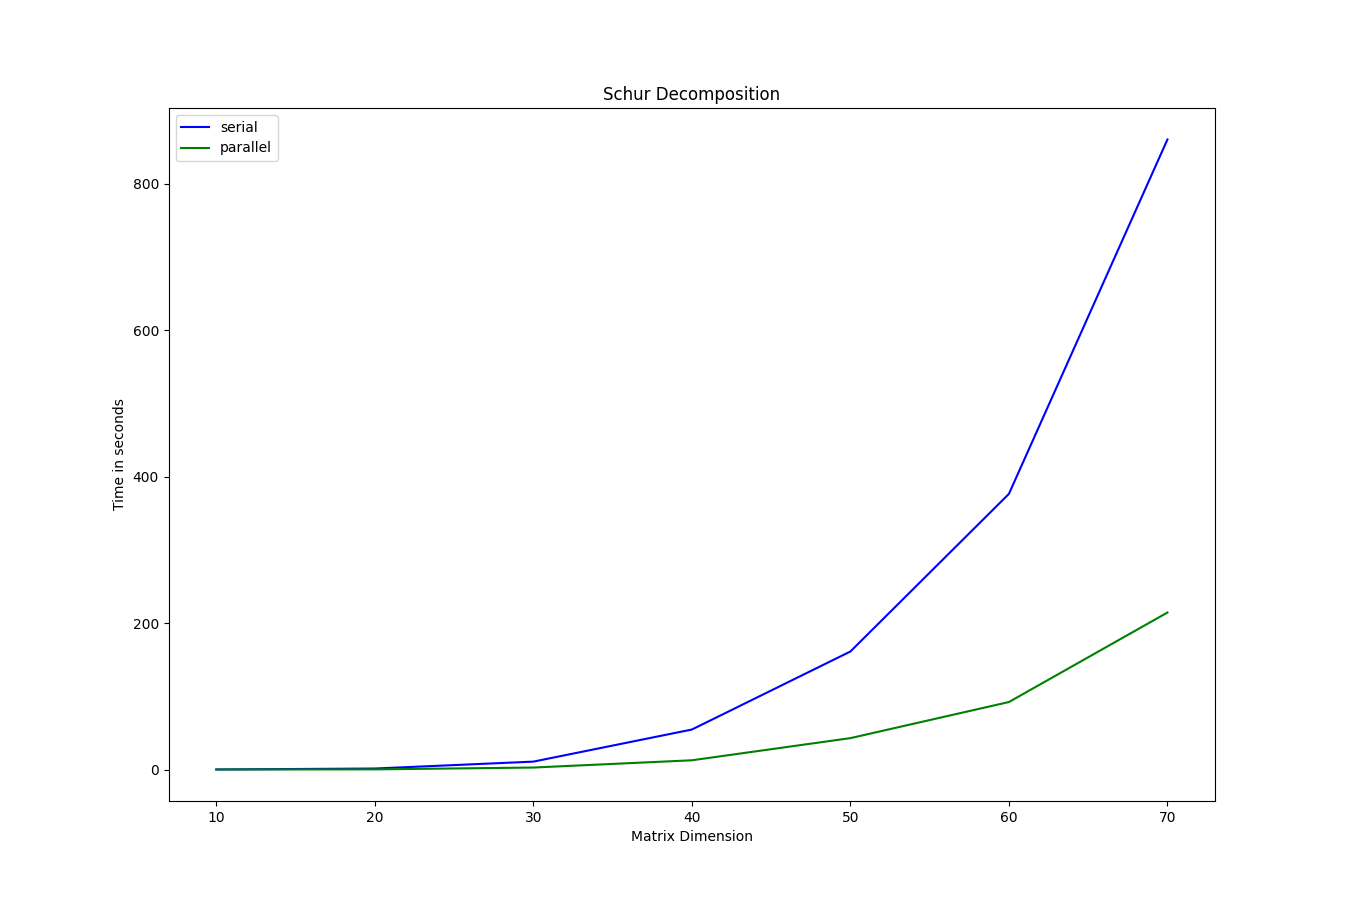
\includegraphics[width=1\textwidth]{schur.png}
    \caption{Order of Execution of schur decomposition}
\end{figure}
\begin{figure}[h]
    \centering
    \includegraphics[width=1\textwidth]{patersonStockmeyer.jpeg}
    \caption{Order of Execution of Paterson Stockmeyer}
\end{figure}


\begin{figure}[!htb]
    \centering
    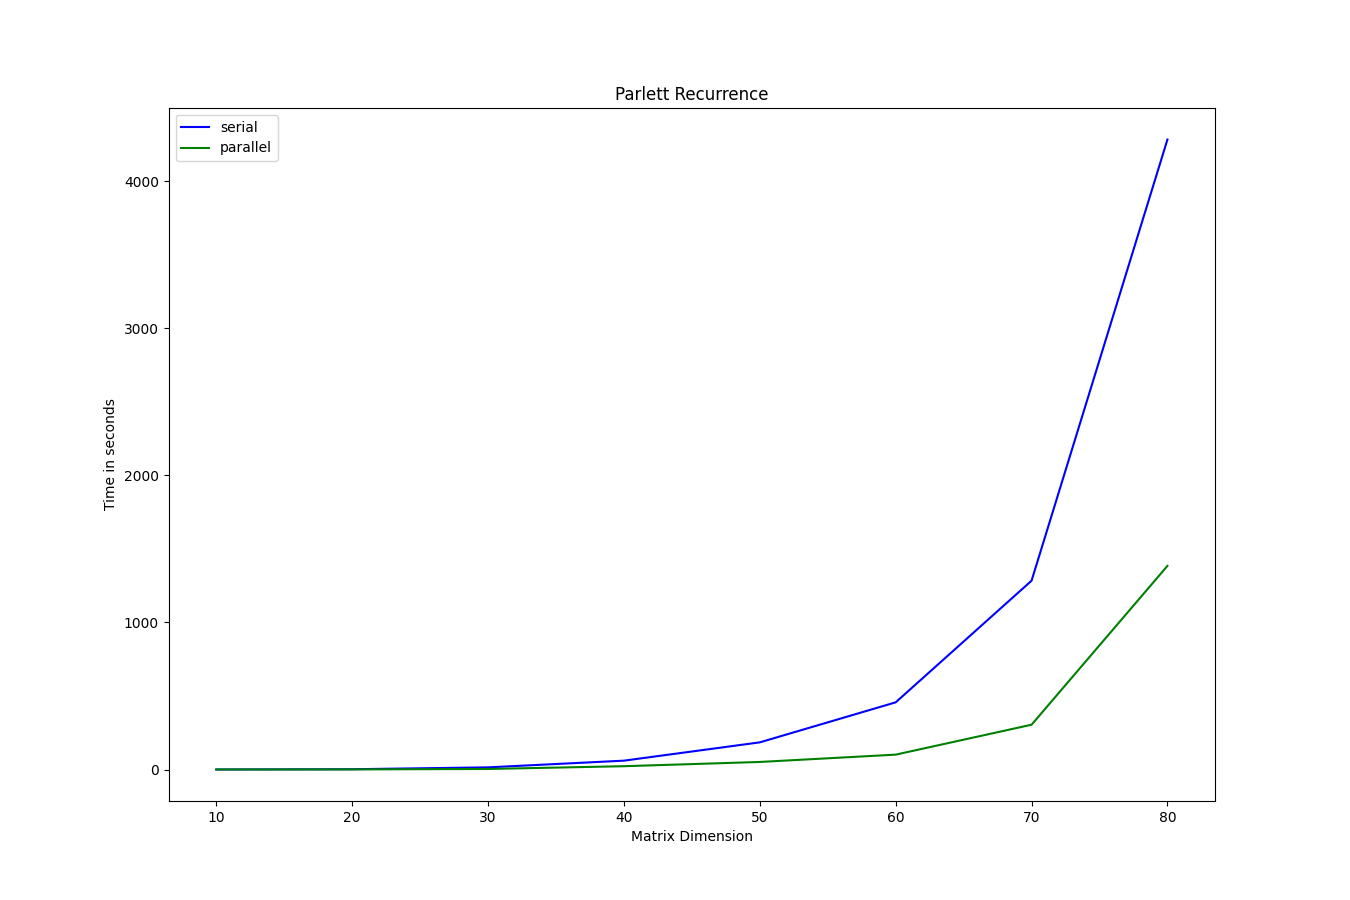
\includegraphics[width=1\textwidth]{parlett.png}
    \caption{Order of Execution of Parlett Recurrence}
\end{figure}


\begin{figure}[h]
    \centering
    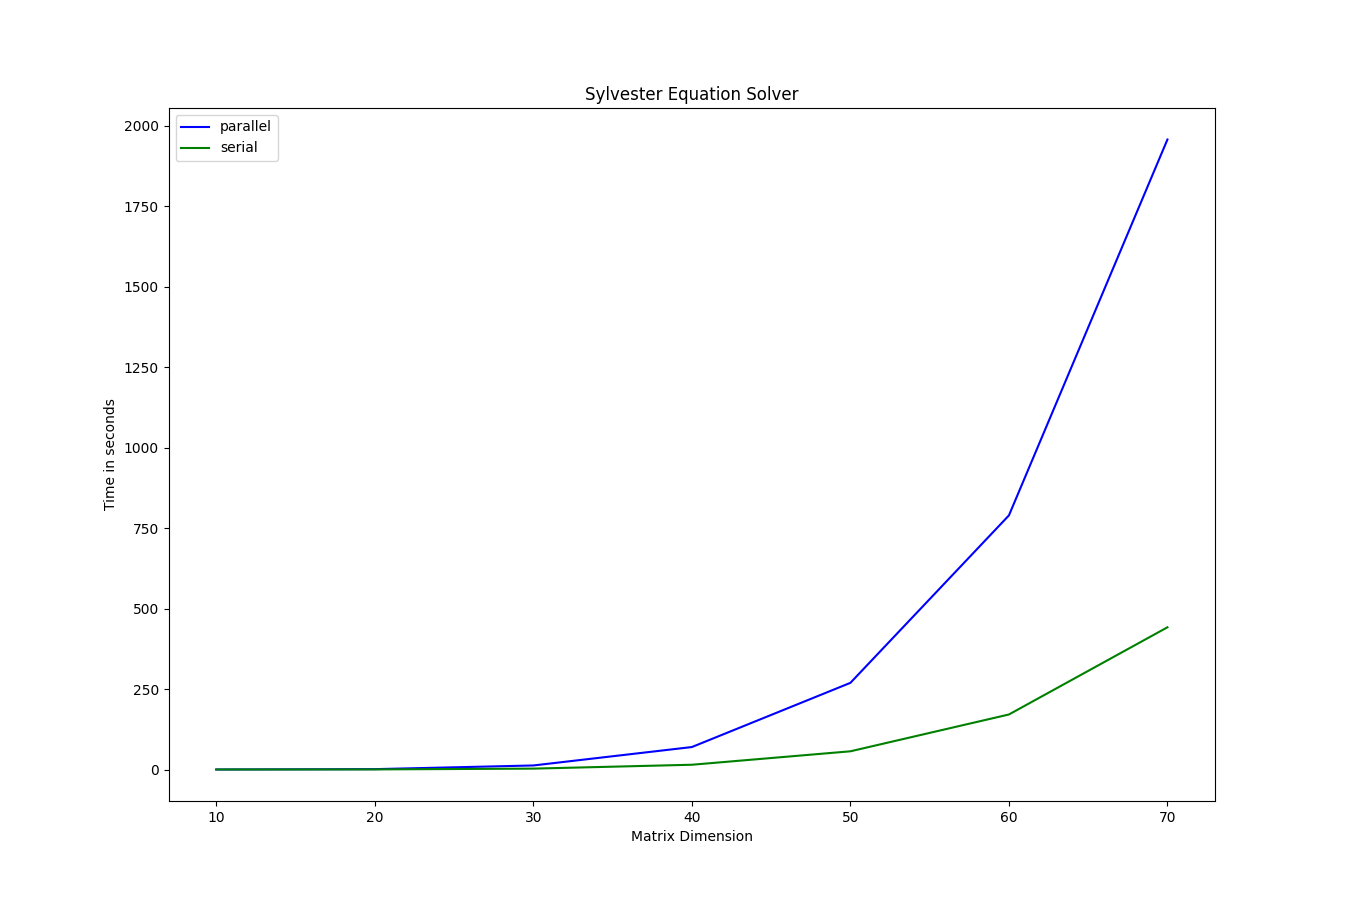
\includegraphics[width=1\textwidth]{sylvester.png}
    \caption{Order of Execution of Sylvester}
\end{figure}


\newpage     
\section{Conclusion}

We have proposed two optimal algorithms for evaluating matrix polynomials. Paterson Stockmeyer is a robust algorithm with time complexity $O(n^3\sqrt{d})$. We explained the sub-components of this method which includes computing of powers of $A$ till $p$ and Horner's method. We also gave a parallelized solution for the same. We also gave another method Parlett Recurrence method which is asymptotically better because it has time complexity $O(n^3)$. But, the constant term for the same is very high and it fails on some edge cases too. Parlett Recurrence comprises of two sub-routines Schur Decomposition and Sylvester Equation Solver. For Schur Decomposition, we chose $QR$ method and for $QR$ decomposition, we are using Given's rotations. We have also gave various optimisations and parallelisation techniques for the same. We used Gauss Elimination for solving Sylvester Equation and also parallelized it. Finally, in Parlett Recurrence we propose a diagonal block partitioning method and we also parallelized it. At last, we evaluated our model and we found the speedup to be about 4X for both Paterson Stockmeyer and Parlett Recurrence even for matrices with relatively smaller dimensions and polynomials with relatively lower degree. We predict that the performance will be better for even larger matrices and higher degree polynomials but we have kept that for future developments of the project due to limitation of access to computing power.


\newpage

%===========================================================
%===========================================================

\bibliographystyle{ieeetr}
\bibliography{refs}
\begin{thebibliography}{9}
\bibitem{sivan}
Sivan Toledo and Amit Waisel: Parallel Algorithms for Evaluating Matrix Polynomials
\bibitem{texbook}
Amit Waisel: Parallell algorithms for evaluating matrix polynomials. Master’s
thesis, School of Computer Science, Tel-Aviv University, 2019.
\bibitem{wiki}
Wikipedia: Schur decomposition
\bibitem{wiki1}
Wikipedia: QR Algorithm
\bibitem{wiki2}
Wikipedia: Givens Rotation
\bibitem{wiki3}
Wikipedia: QR Decomposition
\bibitem{block}
Isak Jonsson, Bo Kagstrom: Recursive Blocked Algorithms for Solving Triangular Systems—Part I: One-Sided and Coupled Sylvester-Type Matrix Equations
\bibitem{schurfor}
Daniel Kressner: Block Algorithms for reordering standard and generalized schur forms Lapack working note 171

\end{thebibliography}


\end{document} 
